\section{Summaries}

Summaries are used to represent and describe the information contained in datasets. They csan be graphical summaries, which visually represent the data, or numerical summaries, which give a description of the data in terms of numbers.

\subsection{Graphical summaries}
\paragraph{Empirical CDF} A random variable is completely characterized by its CDF. We can approximate the CDF with the empirical cumulative distribution function, which is defined as
\begin{equation*}
    F_n(x) = \frac{|\{ i : [1,n] | x_i \leq x \}|}{n}
\end{equation*}
where the $x_i$ are the observations in the dataset. The \textbf{Glivenko-Cantelli theorem} states that the empirical CDF converges to the true CDF as $n$ goes to infinity:
\begin{equation*}
    P(\lim_{n \to \infty} \sup_x |F(x) - F_n(x)| = 0) = 1
\end{equation*}
This approximation can be plugged into different formulas to estimate other quantities, such as the mean or the variance.

\paragraph{Bar plots and histograms}
A bar plot is used for discrete data. It provides a frequency count for the values in the dataset, and approximates the PMF (as a consequence of the law of large numbers, as seen in a previous example):
\begin{equation*}
    P(X = a) \approx \frac{|\{ i | x_i = a \}|}{n}
\end{equation*}
A histogram is used for continuous data. It provides frequency counts for ranges of values (instead of individual ones). The support of the random variable is first split into $m$ intervals called \textbf{bins} (which can all have the same width or different widths), and the number of occurrences belonging to each bin is counted and normalized:
\begin{equation*}
    A_i = \frac{|\{ j \in [1,n] |x_j \in B_j\}|}{n} \approx P(X \in B_i)
\end{equation*}
The bins can be plotted as rectangles so that their area is proportional to $A_i$; after fixing their width $b_i$, the height is found as $H_i = A_i / b_i$.

Bin width can be chosen in different ways, producing different results. It is common to choose the same width for all bins, such that, for a total number of bins $m$, the interval corresponding to the $i^{th}$ bin is
\begin{equation*}
    B_i = (r + (i-1)b, r + i*b)
\end{equation*}
where $r$ is the minimum value taken by the random variable, and $b$ is the bin width. The optimal width can be found using \textbf{Mean Integrated Squared Error} (\textbf{MISE}):
\begin{equation*}
    MISE = \E \left [ \int (\hat{f}(t) - f(t))^2 \ dt \right ] = \int \int (\hat{f}(t) - f(t))^2 f(x_1) \ldots f(x_n) \ dt dx_1 \ldots dx_n
\end{equation*}
where $\hat{f}$ is the density estimation of the real PDF $f$. The minimum of the MISE for Normal distributions is represented by \textbf{Scott's normal reference rule}:
\begin{equation*}
    b = 3.49 \cdot s \cdot n^{-1/3}
\end{equation*}
wher $s$ is the sample standard deviation.\\
Other options are:
\begin{itemize}
    \item \textbf{Freedman-Diaconis' choice}:
    \begin{equation*}
        b = 2 \cdot \text{IQR} \cdot n^{-1/3}
    \end{equation*}
    This choice is more robust to outliers than the previous.
    \item \textbf{Variable bin width} (such as logarithmic binning as seen in power-law distributions).
    \item \textbf{Fixing the number of bins, and derivaring the width from it}. Some common strategies are:
    \begin{align*}
        &m = \lceil \frac{\max x_i - \min x_i}{b} \rceil\\
        &m = \lceil \sqrt{n} \rceil\\
        &m = \lceil \log_2 n \rceil + 1 \text{ (Sturges' rule)}
    \end{align*}
    The latter assumes normal distribution for the true density. This distribution can be approximated by a $Bin(n, 0.5)$ distribution, so the absolute frequency of the $i^{th}$ bin is $\binom{m-1}{i}$. The total frequency is $n = \sum_{i=0}^{m-1} \binom{m-1}{i} = 2^{m-1}$, from which $m$ is derived.
\end{itemize}

\paragraph{Kernel density estimation}
A big disadvantage of histograms is that the result strictly depends on the number of bins/bin width chosen to visualize the data. Kernel density estimation is another popular method to summarize distributions which is not as sensitive to the choice of parameters.

The idea behind this method is to mix kernel functions (which can take different forms, see Fig \ref{fig:kernels}) centered in each observation in the dataset. Since data is assumed to be of continuous nature, the presence of a certain value in the dataset also contributes to the density of the values around it. The kernel function models the way this density is distributed around that single observation, and by mixing together all the kernels, the result should be a good approximation of the true density.
\begin{figure}[h]
    \centering
    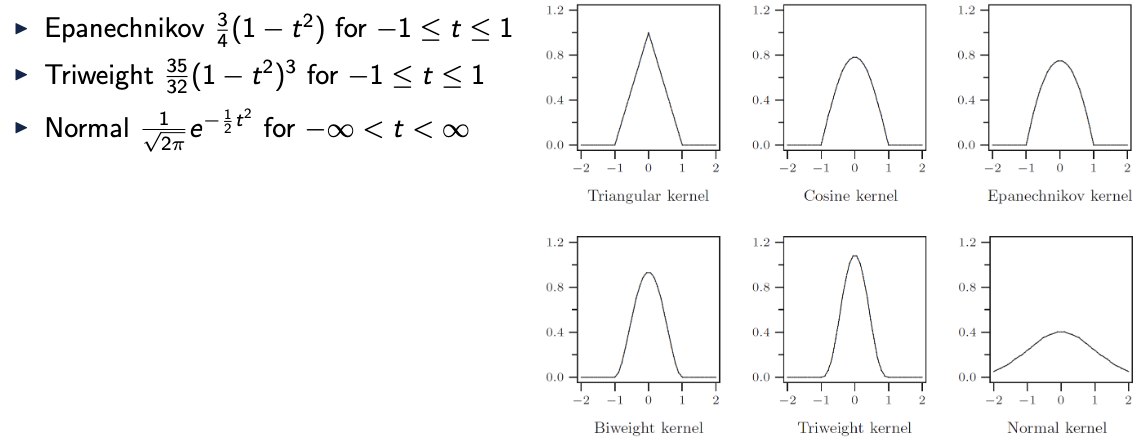
\includegraphics[width=0.8\textwidth]{img/kernels.png}
    \caption{Examples of common kernels used in KDE.}
    \label{fig:kernels}
\end{figure} \\
\boxdefinition{Kernel}{
    A kernel is a function $K : \mathbb{R} \to \mathbb{R}$ such that
    \begin{itemize}
        \item $K$ is a probability density: $K(t) \geq 0$ and $\int_{-\infty}^{\infty} K(t) \ dt = 1$
        \item $K$ is symmetric: $K(-t) = K(t)$
        \item $K(t) = 0$ for $|t| > 1$ (i.e., support is $[-1, 1]$)
    \end{itemize}
}
The last requirement is not strictly necessary, actually; for example, the Normal kernel has unbounded support.

Each kernel function is characterized by a center (the observation), and a \textbf{bandwidth} $h$, which is a scaling factor over the support of the kernel from $[-1, 1]$ to $[-h, h]$. In other words, the badwidth determines how tall-thin or short-wide the kernel is around its center. We can then write
\[
    X \sim K(t) \implies h \cdot X + x_i \sim \frac{1}{h} K \left ( \frac{t - x_i}{h} \right )
\]
because of the change-of-units transformation formulas. The final kernel density estimate is the result of the \textbf{mixture} of all the scaled and shifted kernel densities:
\begin{equation*}
    f_{n,h} (t) = \frac{1}{nh} \sum_{i=1}^n K\left ( \frac{t-x_i}{h}\right )
\end{equation*}
The $1/n$ in the formula is a normalization factor that ensures the density integrates to 1.

The choice of kernel is not critical to the final result; different kernels behave similarly. The key parameter is the bandwidth $h$. Also for KDE, MISE can be used to find the optimal value. Assuming the true density is Normal, the MISE is minimized for
\begin{equation*}
    h = \left (\frac{4}{3} \right )^{1/5} \cdot s \cdot n^{-1/5}
\end{equation*}
For other distributions, the optimal bandwidth can be found using plug-in selectors or cross validation selectors.

Another issue that may arise is when the support of the random variable is bounded. If KDE is used as is, the result will present density event corresponding to values that are not possible. To avoid this, boundary correction techniques are used; some examples are
\begin{itemize}
    \item Kernel truncation and renormalization (forced truncation of the kernel outside the support);
    \item Linear combination kernel;
    \item Beta boundary kernels;
    \item Reflective kernels.
\end{itemize}

\subsection{Numerical summaries}

\paragraph{Sample summaries} Summaries of the empirical data can be used to estimate summaries of the true distribution. The following are some common ones:
\begin{itemize}
    \item \textbf{Sample mean}:
    \begin{equation*}
        \bar{x} = \frac{x_1 + \ldots + x_n}{n}
    \end{equation*}
    \item \textbf{Median}:
    Let $x_1, x_2, \ldots, x_n$ be the data in the sample, sorted.
    \begin{equation*}
        Med(x_1, \ldots, x_n) = \begin{cases}
            x_{n/2} &\text{if } n \text{ is odd}\\
            \frac{x_{n/2} + x_{n/2 + 1}}{2} &\text{if } n \text{ is even} 
        \end{cases}
    \end{equation*}
    The median of a distriution corresponds to the $0.5^{th}$ quantile.
    \item \textbf{Sample variance and standard deviation}:
    \begin{align*}
        &s_n^2 = \frac{\sum_i^n (x_i - \bar{x_n})^2}{n-1} & s_n = \sqrt{s_n^2}
    \end{align*}
    \item \textbf{Median of absolute deviations}:
    \begin{equation*}
        MAD(x_1, \ldots, x_n) = Med(|x_1 - Med(x_1, \ldots, x_n)|, \ldots, |x_n - Med(x_1, \ldots, x_n|))
    \end{equation*}
    If the distribution is symmetric, the MAD is exactly equal to the difference between the $0.75^{th}$ and $0.5^{th}$ quantiles.
\end{itemize}

\paragraph{Order statistics} Let $x_1, x_2, \ldots, x_n$ be the ordered sequence of values in a sample. $x_{\langle i \rangle}$ is the $i^{th}$ order statistic. Order statistics are used to calculate empirical quantiles. Formally, the $p^{th}$ quantile is the value $q_p$ such that $q_p = \inf_x \{ P(X \leq x) \geq p \} = \inf_x \{F(x) \geq p\}$ (to be read as: ``the smallest number $x$ such that the probability of $X$ being less or equal than $x$ is greater or equal than $p$''). To find the empirical quantiles, we use the empirical approximation of the CDF in place of the true CDF:
\[
    q_p = \inf_x \{ F_n(x) \geq p \} = \inf_x \left\{\frac{|\{i | x_i \leq x \}|}{n} \geq p \right\}
\]
There are actually many ways to find the quantiles of a distribution. In \texttt{R}, there are 9 variants. The default one is type 7:
\begin{equation*}
    p = \frac{i-1}{n-1} \implies q_p = x_{\langle p\cdot(n-1) + 1 \rangle}
\end{equation*}
Another common choice is type 6:
\begin{equation*}
    p = \frac{i}{n+1} \implies q_p = x_{\langle p \cdot (n+1) \rangle}
\end{equation*}
The difference between the methods is irrelevant for big enough datasets.

What if the supposed index of the quantile is not an integer? In this case, the quantile is approximated using linear interpolation. Let $k = \lfloor p \cdot (n+1) \rfloor$ (or whatever other formula is used by the chosen method). Then,
\begin{equation*}
    q_p = x_{\langle k \rangle} + \alpha \cdot (x_{\langle k+1 \rangle} - x_{\langle k \rangle})
\end{equation*}
where $\alpha = p \cdot (n+1) - k$, i.e., the decimal part of the index.

\paragraph{Association and correlation}
\textbf{Association} measures how much information one variable provides on another. If two variables are independent, they are not associated. Association is maximum when one variable is a (invertible) function of the other. \textbf{Correlation} measures the presence and strenght of an increasing/decreasing trend between two variables. If two variables are independent, their correlation is always 0, but the opposite is not always true.
\boxdefinition{Correlation}{
    Let $X$ and $Y$ be two random variables. The correlation coefficient $\rho$ is defined to be 0 if $Var(X) = 0$ or $Var(Y) = 0$, and otherwise as
    \begin{eqnarray}
        \rho = \frac{Cov(X, Y)}{\sqrt{Var(X) \cdot Var(Y)}}
    \end{eqnarray}
}
Some common correlation coefficients are:
\begin{itemize}
    \item \textbf{Pearson's r}: it is obtained by substituting the sample covariance and the sample standard deviations of the random variables in the formula above:
    \begin{align*}
        &s_{xy} = \frac{\sum_{i=1}^n (x_i - \bar{x}) \cdot (y_i - \bar{y})}{n-1} &r = \frac{s_{xy}}{s_x \cdot s_y}
    \end{align*}
    It is bounded in the interval $[-1,1]$. The computational cost to calculate it is $O(n)$. A limitation of Pearson's r is that it can only detect linear relationships between random variables, and it can only be used when the variables are continuous.
    \item \textbf{Spearman's $\rho$}: this coefficient is calculated as the correlation between ranks of the observations. Let $\textit{rank}(x)$ be the ranks of the values of the variable $x$. Then, Spearman's $\rho$ is calculated as
    \begin{equation*}
        \rho = r(\textit{rank}(x), \textit{rank}(y)) = 1 - \frac{6 \sum_{i=1}^n (rank(x)_i - rank(y)_i)^2}{n\cdot(n^2 - 1)} 
    \end{equation*}
    This coefficient assesses monotonic relationships of any kind (both linear and non-linear). The computational cost to calculate it is $O(n \cdot \log n)$, since it requires a sorting of the data to compute the ranks. It can be used when both variables are ordinal, continuous, or when one is ordinal and the other is continuous.
    \item \textbf{Kendall's $\tau$}: this coefficient compares the sign of the differences between successive pairs of observations. It is calculated as
    \begin{equation*}
        \tau_a = \frac{2 \sum_{i<j} \textit{sign}(x_i - x_j) \cdot \textit{sign}(y_i - y_j)}{n \cdot (n-1)}
    \end{equation*}
    It calculates the fraction of concordant pairs minus discordant pairs of values between the two variables, and it is bounded in the interval $[-1,1]$. The computational cost to calculate it is $O(n^2)$. There is a variant, $\tau_b$, which also takes into account the possibility of ties; instead of dividing by $n \cdot (n-1)$, it counts how many pairs do not present a tie in $x$ or $y$. It can be used when both variables are ordinal, or when one is ordinal and the other is continuous.
    \item \textbf{Somer's D}: this coefficient is used when one variable is continuous and the other is binary. It can be seen as an asymmetric version of Kendall's $\tau$:
    \begin{eqnarray}
        D = \frac{\tau_{xy}}{\tau{yy}} = \frac{\sum_{i<j} \textit{sign}(x_i - x_j) \cdot \textit{sign}(y_i - y_j)}{\sum_{i<j} \textit{sign}(y_i - y_j)^2}
    \end{eqnarray}
    It calculates the fraction of concordant pairs minus discordant pairs over the number of unequal pairs of values in $y$. An example application can be seen with probabilistic classifiers: $x$ is the confidence prediction of an example being positive, $y$ is the true class, and $D$ is the Gini index of the classifier.
    \item \textbf{Thiel's U}: it is used when both variables are nominal. It can be calculated in a symmetric and an asymmetric way:
    \begin{align*}
        &U_{sym} = \frac{2 \cdot I(X,Y)}{H(X) + H(Y)} &U_{asym} = \frac{I(X,Y)}{H(X)}
    \end{align*}
    where $I(X,Y)$ is the mutual information between $X$ and $Y$, and $H(X), H(Y)$ are the entropies of the two random variables. The asymmetrical version, specifically, indicates what fraction of $X$ can be predicted by $Y$.
\end{itemize}